\chapter{\textbf{INTRODUCTION}}\label{Introchap} 
%\chapter{\normalsize \textbf{CHAPTER 1}}} \label{Introchap}

\section{Background}

We are living in a world where technology advancement as continuous phenomena: new applications and devices introduced every now and then such as social media, internet banking, e-commerce, massive open online courses (mooc) , smart-phone, tab, ipad, wearable sensors, self-driving car and etc. These new applications and devices which are important aspect of our daily activities creates massive data \cite[]{torrecilla2018data}. Learning from these data is important for decision making and to improve the process and productivity. 

However raw data are often large, making learning from these are almost impossible. Data must be organized, summarized and described in the form that facilitate us to gain information and knowledge. Descriptive statistics which is one of the major two branches of statistic is commonly used to explore the data before any statistical test performed known as inferential statistics. 

Exploratory Data Analysis (EDA) is one of the method used in descriptive statistics. EDA was introduced by John W. Tukey in 1977 \cite[]{wendy2002computational}. EDA is mostly involves statistical graphs, is an approach of analyzing data visually without a prior assumptions on parametric model of the data, error terms, outliers in data, modality of the data and relationship with other variables \cite[]{velleman1981applications,wendy2002computational}. Visualising data is vital in exploring data \cite[]{scott2005multidimensional} to help in finding the  patterns, structure in data and relationships between variables in data \cite[]{hand2001principles}. EDA helps the researchers to model data based on the what is revealed through exploring with various graphical methods. Generally after the EDA process one would use confirmatory analysis such as hypothesis testing, ANOVA, regression and etc.

Histogram is one of the important tools used in EDA. It is used often in graphical analysis to visualise data \cite[]{li2016essential}. The subject of histogram is so important that it is included in every elementary statistics or data analysis course. 

\section{Histogram}

Histogram useful in summarising large amount numerical data graphically \cite[]{kirschenmann2015note} and to visualise the distribution of data without prior assumptions on the characteristics of data or the underlying true distribution of the data. Hence histogram is called as a non-parametric density estimator\cite[]{keen2010graphics}. Once a histogram is constructed the general attributes of the data such as symmetry, modality, central location and spread of the data will be revealed.

A typical histogram is a stack of rectangular columns each of whose heights is proportional to the corresponding frequency of data values. Data values grouped into intervals, called as bins (or classes). In constructing histogram number bins or equally the bin width must be decided upfront. Bins can be either same size (i.e equal width) or different size (i.e unequal width) provided it should encompass all the data and non overlap with each other. Number of bins used to construct histogram will determines the shape of it. Too many bin makes the histogram uneven and unable to find the underlying trend of the data. Too few bin gives little information about the data. 

\section{Histogram Bins}

Number of bins in grouping data can be predefined upfront or using some scientific rules. For example data on marks in a exam can be grouped into 5 bins: 0-20, 20 - 40, 40-60, 60-80 and 80-100. Alternatively one can use rules such Sturges(1926) rule as a guide to decide number of bins. For sample data of size 40, the Sturges(1926) rule suggest 7 bins. More discussion on rules in Chapter 2 - Literature Review.

%Most statistical packages default settings uses Sturges' rule in calculating number of bins. Herbert Sturges(1926) proposed a simple rule for classifying a series of n items. %The expectation is that a normally distributed variable can be appropriately divided so that the bin frequencies comprise a binomial series for all n which are powers of 2. 
%Doane (1976) provide a modification to Sturges' rule which attempts to improve its construction of histogram with skewed data. Beside Doane (1976), Scott's (1979) and Freedman and Diaconis's (1981) gives alternative rules for constructing histogram by the bin width. 


\section{Numerical Data }

Numerical data can be classified into discrete and continuous data. 

A set of data is said to be discrete if the values belonging to the data set only assumes integer values as 0,1,2,3,4 and etc. There are gaps between two possible values in a discrete dataset. Examples of discrete data are number of children in a family, number of cars on the road, number of students in a school, number of defective items and etc.

Continuous data assumes any values between two specific values. Continuous data are normally obtained by measuring. There are no gaps in between any two possible values in a continuous dataset. Examples of continuous data are height of students in an university, amount of rain in a month, volume of water (in ml) in a bottle, and etc. 

\section{Raw Data and Grouped Data}
 
Dataset can be presented as raw (ungrouped) or grouped data. Raw data is usually unsorted are given as list of data values in the dataset. Grouped data is the raw data that has been sorted into a set classes or intervals or bins. While discrete data can be summarised using a frequency table continuous data must grouped in a set of bins before the frequency table can produced.


\section{Frequency}

Frequency is simply counts of a data value appears in a given dataset.  Frequency of a dataset displayed using a table format known as frequency table based on the classes or bins. Obtaining  frequency of dataset is the first step in summarising dataset before producing graphical charts for visualisation.




\section{Frequency Table}




\section{Frequency Polygon}

\section{Bar Chart}

\section{Use of Histogram}

Histogram can provide a clue to researchers of a possible parametric model suitable for data  \cite[]{wendy2002computational} besides detecting unusual observations or behavior in data. Histogram can be used to estimate the 5 number summary of data and variation in data.

Histogram is widely used as one of the Seven (7) Quality Control Tools (7QC) to ensure manufacturing process are within the controlled specification or to maintain the quality level \cite[]{magar2014application}. 


Histogram based image processing that is very useful for medical image analysis, industrial X-ray and etc is used widely because easy to understand and implement besides being effective \cite[]{sharma2015review}.


Regression with Histogram Data.

\section{Problem Statement}

Deciding how many bins to be used is still a challenge to most researchers especially when background of the data is unknown. Despite there many suggested methods to determine the number of bins, there is no single method is agreed upon. The five number summary and variation calculated from raw data can used in deciding the number bins.

Detecting the outliers from histogram not very helpful due the method of constructing. The modification of construction histogram can reveal the outliers more effectively.


\section{Research Aims and Objectives}

This study aims to achieve following objectives:

\begin{itemize}
	\item propose a method using raw data five number summary and variation to decide the number of bins.
	\item evaluate new method with existing methods
	\item propose a new method for construction of histogram to detect outliers
	\item evaluate new method against box-plot method to detect outliers
	\item propose a fixed frequency histogram for the purpose of segmentation 

\end{itemize}



\section{Limitation of Study}

\section{Structure of Thesis}


\addblankpage % disable this if the last page for this chapter is even

\chapter{\textbf{LITERATURE REVIEW}}\label{Introchap} 
%\chapter{\normalsize \textbf{CHAPTER 1}}} \label{Introchap}

\section{History of Histogram}

The term "histogram" was introduced by Karl Pearson \cite[]{ross2010introductory, rufilanchas2017origin} but there was confusion on the date or year it was introduced \cite[]{rufilanchas2017origin,ioannidis2003history}. Several authors stated the year as 1895 \cite[]{beniger1976history, dodge2008concise,ross2010introductory,li2016essential}. However \cite[]{magnello2014introducing, rufilanchas2017origin} clarified that the histogram was first introduced in 1891 in Gresham Lectures. Karl Pearson used the term while lecturing on "Maps and Chartograms" \cite[]{rufilanchas2017origin}.

Beside confusion on year of the term "histogram" was introduced there is also some confusion on the meaning of "histogram". The term is frequently misunderstood that it is used to study history \cite[]{rufilanchas2017origin}.  The association of histogram as historical diagram was due to the fact that Karl Pearson use time histogram in his lecture to describe the "time-diagram" but he do not meant histogram used to study the subject "history" \cite[]{rufilanchas2017origin}.

Histogram has been used long before it received its name i.e from seventeen century. \cite[]{scott1979optimal,loquin2008histogram} believes that John Graunt (as cited in Westergard , 1968, p.22) probably was using histogram in 1662. John Graunt(1662) used a histogram to describe the mortality rate \cite[]{copas1983non,scott2005multidimensional}.  However \cite[]{chen2007handbook,ross2010introductory,rufilanchas2017origin} believes that William Playfair (1759- 1823) who invented bar chart was the person responsible in introducing histogram in 1801.  

Andre-Michael Guerry (A.M Guerry) a French mathematician was also given credit in introducing histogram in 1833 when he use William Playfair's bar chart concept on continuous data by categorizing i.e data on age and time. \cite[]{beniger1976history,friendly2007m,ross2010introductory}. A.M. Guerry produced his first publication in 1829 about crime in France population. In 1833 he return with his second publication by refining and extending data on his first published work. His third and major work that happened in 1864. Third publication used histogram as one of the main tool in presenting the comparison of crime against population between France and England \cite[]{friendly2007m}.

According to \cite[]{ross2010introductory} the systematic development in histogram was due to the work of Adolphe Quetelet in 1846 where he introduce methodological steps in doing research. Quetelet who was a Belgian statistician gave importance to graphical visualization for social science researches. Since then the histogram was further developed such as comparing data from different categories. For example Francis A. Walker[1840-1897] in producing the Atlas of Ninth Census for U.S nationals in 1874 incorporated a bilateral histogram to show graphically the distribution of deaths by sex and month of death and according to race and nationality \cite[]{beniger1976history, friendly2008golden}. 

Despite being one of the oldest graphical display tool, histogram is still being relevant for presenting univariate continuous data  visually \cite[]{scott1979optimal, wand1997data} and also being used in recent "Big Data Analytics" \cite[]{berger2016big}.

\addblankpage % disable this if the last page for this chapter is even

\chapter{\textbf{METHODOLOGY}}\label{Introchap} 
%\chapter{\normalsize \textbf{CHAPTER 1}}} \label{Introchap}

%\section{Variations on the Histogram}
%
%One of the histogram use: it's a nonparametric density estimator for an underlying true density function $f(x)$ \cite[]{waterman1978estimation,scott1979optimal} besides being useful for summarising and visualising data. We know from calculus that for any continuous variable $X$, the area under density function must be equal to one, a principle based on probability. 
%
%\begin{equation}
%\int_{- \infty}^{\infty} f(x) \, dx = 1 , f(x) \geq 0
%\end{equation}
%
%\begin{figure}[h]
%	\caption{Density Plot}
%	\centering 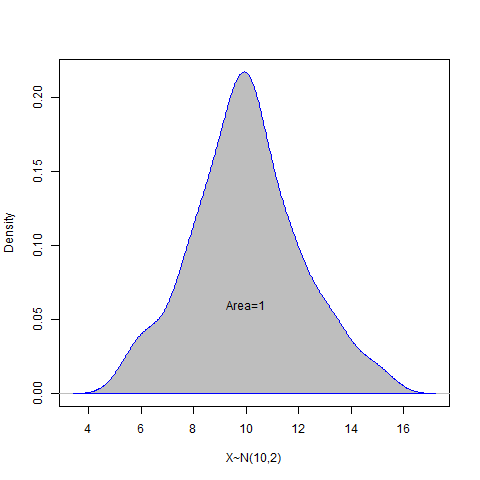
\includegraphics[scale=0.5]{density}
%\end{figure}
%
%Same principles applies to the histogram being empirical density estimator: the area under represented by histogram must be equal to one. 
%
%\begin{figure}[h]
%	\caption{Histogram with Density Plot}
%	\centering 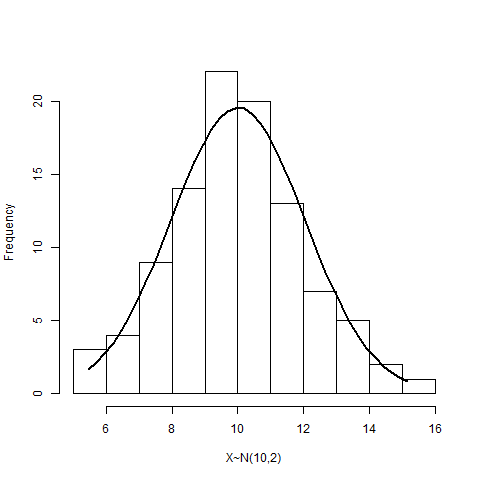
\includegraphics[scale=0.5]{hist_density}
%\end{figure}
%
%\clearpage
%
%As such any variation in histograms must satisfy this principles at all time. 

%\subsection{Equal width Histogram}


The most common histogram found and being used to explore the distribution of data. Each bin in equal width and non overlap.

\begin{figure}[h]
	\caption{Equal Width Histogram}
	\centering 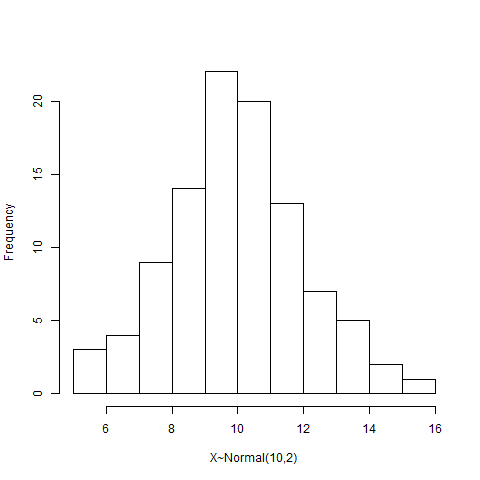
\includegraphics[scale=0.5]{hist_equalwidth}
\end{figure}

\section{Classical Histogram}
\subsection{Flow of Constructing Histogram}
\begin{enumerate}
	\item Selecting Bin Width
	\item Selecting Starting Point for First Bin
	\item Constructing the frequency Table
	\item Constructing the Histogram
\end{enumerate}

\begin{enumerate}
	\item Selecting Number of Bin
	\item Selecting Starting Point for First Bin
	\item Constructing the frequency Table
	\item Constructing the Histogram
\end{enumerate}
\subsection{Selection of Bins}

\subsection{Equal Width}

\subsection{Unequal Width}

\subsection{Symmetrical Data}

\subsection{Heavy Tail Data}
 
\subsection{Big Data and Small Data}
\subsection{Missing Data}
 

Frequency Table



compare the distribution with normal,

\section{Selecting the Best Histogram Representing Data}
\subsection{Goodness of Fit for Histogram}
\subsection{Statistics from frequency table}
\section{Modification of Constructing Histogram}

\subsection{Modification via Bin Numbers}

\subsection{Modification Via Bin Width}

\subsection{Modification for Heavy Tail Data}

\subsection{Starting point of constructing the histogram}

\section{Handling Big Data with Histogram}

\section{Histogram by Area}


\section{Modification  of Histogram} 
\subsection{Mode Formula}
\subsection{Mean Formula}
\subsection{Kurtosis}

\section{Histogram by Area\ Fall Down(Order Frequency Histogram)}

\section{Percentile Histogram}


\addblankpage % disable this if the last page for this chapter is even
